\documentclass[UTF-8,twoside,cs4size]{ctexart}
\usepackage[dvipsnames]{xcolor}
\usepackage{amsmath}
\usepackage{amssymb}
\usepackage{geometry}
\usepackage{setspace}
\usepackage{xeCJK}
\usepackage{ulem}
\usepackage{pstricks}
\usepackage{pstricks-add}
\usepackage{bm}
\usepackage{mathtools}
\usepackage{breqn}
\usepackage{mathrsfs}
\usepackage{esint}
\usepackage{textcomp}
\usepackage{upgreek}
\usepackage{pifont}
\usepackage{tikz}
\usepackage{circuitikz}
\usepackage{caption}
\usepackage{tabularx}
\usepackage{array}
\newcolumntype{Y}{>{\centering\arraybackslash}X}
\usepackage{pgfplots}
\usepackage{multirow}
\usepackage{pgfplotstable}
\usepackage{mhchem}
\usepackage{physics} % Add this package for \dt and \dif commands
\usepackage{cases}
\usepackage{subfigure}
\usepackage{enumerate}
\usepackage{minipage-marginpar}
\usepackage{diagbox}
\usepackage{graphicx}


\graphicspath{{./figure/}}

\setCJKfamilyfont{zhsong}[AutoFakeBold = {5.6}]{STSong}
\newcommand*{\song}{\CJKfamily{zhsong}}

\geometry{a4paper,left=2cm,right=2cm,top=0.75cm,bottom=2.54cm}

\newcommand{\experiName}{磁场的测量}%实验名称
\newcommand{\supervisor}{全保刚}%指导教师
\newcommand{\name}{孙奕飞}
\newcommand{\studentNum}{2023k8009925001}
\newcommand{\class}{2}%班级
\newcommand{\group}{06}%组
\newcommand{\seat}{01}%座位号
\newcommand{\dateYear}{2024}
\newcommand{\dateMonth}{12}%月
\newcommand{\dateDay}{3}%日
\newcommand{\room}{教708}%地点
\newcommand{\others}{$\square$}

\ctexset{
    section={
        format+=\raggedright\song\large
    },
    subsection={
        name={\quad,.}
    },
    subsubsection={
        name={\qquad,.}
    }
}

\begin{document}
\noindent

\begin{center}

    \textbf{\song \zihao{-2} \ziju{0.5}《基础物理实验》实验报告}
    
\end{center}


\begin{center}
    \kaishu \zihao{5}
    \noindent \emph{实验名称}\underline{\makebox[28em][c]{\experiName}}
    \emph{指导教师}\underline{\makebox[9em][c]{\supervisor}}\\
    \emph{姓名}\underline{\makebox[6em][c]{\name}} 
    \emph{学号}\underline{\makebox[14em][c]{\studentNum}}
    \emph{分班分组及座号} \underline{\makebox[5em][c]{\class \ -\ \group \ -\ \seat }\emph{号}} \\
    \emph{实验日期} \underline{\makebox[3em][c]{\dateYear}} \emph{年}
    \underline{\makebox[2em][c]{\dateMonth}}\emph{月}
    \underline{\makebox[2em][c]{\dateDay}}\emph{日}
    \emph{实验地点}\underline{{\makebox[4em][c]\room}}
    \emph{调课/补课} \underline{\makebox[3em][c]{否}}
    \emph{成绩评定} \underline{\hspace{8em}}
    {\noindent}
    \rule[5pt]{17.7cm}{0.2em}
\end{center}

\section{实验目的及实验要求}
1 \textbf{霍尔效应原理及霍尔元件相关参数的含义和作用} \par
2 \textbf{测绘霍尔元件的 $V_H-I_S$ 和 $V_H-I_M$ 曲线,研究霍尔电势差 $V_H$ 与霍尔元件工作电流 $I_S$、磁感应强度 $B$ 以及励磁电流 $I_M$ 之间的关系。} \par
3 \textbf{学习通过霍尔效应测量磁感应强度 $B$ 及磁场的空间分布。} \par
4 \textbf{掌握载流圆线圈磁感应强度的分布规律。} \par
5 \textbf{掌握亥姆霍兹线圈磁感应强度的分布特性。} \par

\section{实验仪器及设备}
\subsection{霍尔效应测量磁感应强度}
1. \textbf{电磁铁磁场}:磁场可调范围为 0~350\,$\mathrm{mT}$,电磁铁励磁电流范围为 0~0.5\,$\mathrm{A}$,连续可调,调节细度优于 1\,$\mathrm{mA}$,稳定性小于 $10^{-5}$,并通过 3 位半数字电压表显示。 \par

2. \textbf{数字式特斯拉计}:测量范围为 0~1000.0\,$\mathrm{mT}$,最小分辨率为 0.1\,$\mathrm{mT}$,配备 4 位半数字电压表显示。 \par

3. \textbf{霍尔工作电流}:调节范围为 0~3.5\,$\mathrm{mA}$,连续可调,最小分辨率为 10\,$\mu\mathrm{A}$,采用 3 位半数字电压表显示。 \par

4. \textbf{霍尔电压表}:测量范围为 0~2.0000\,$\mathrm{V}$,最小分辨率为 0.1\,$\mathrm{mV}$,通过 4 位半数字电压表显示。 \par

5. \textbf{励磁电流及霍尔工作电流}:使用电子换向开关进行切换。 \par

6. \textbf{可调移动尺}:调节范围为 14\,$\mathrm{mm}$~44\,$\mathrm{mm}$。 \par
\subsection{亥姆霍兹线圈的磁感应强度测量}
1. \textbf{亥姆霍兹线圈架} \par

2. \textbf{励磁线圈}:包括两个励磁线圈,单个线圈的直径为 105\,$\mathrm{mm}$。 \par

3. \textbf{线圈匝数}:每个线圈的匝数为实验中预设值(需根据具体型号说明补充)。 \par

4. \textbf{线圈间距}:两线圈中心间距为 105\,$\mathrm{mm}$。 \par

5. \textbf{移动装置}:具有轴向和径向的移动功能,轴向可移动距离为 250\,$\mathrm{mm}$,径向可移动距离为 70\,$\mathrm{mm}$。 \par

6. \textbf{位置测量分辨率}:距离分辨率为 1\,$\mathrm{mm}$。 \par

7. \textbf{DH4501 亥姆霍兹磁场测量仪}: \par
   (1)\textbf{频率范围}:20~200\,$\mathrm{Hz}$,频率分辨率为 0.1\,$\mathrm{Hz}$,测量误差为 0.1\%; \par
   (2)\textbf{正弦波输出}:输出电压幅度最大为 20\,$\mathrm{Vp-p}$,输出电流幅度最大为 200\,$\mathrm{mA}$; \par
   (3)\textbf{数显毫伏表}:电压测量范围为 0~20\,$\mathrm{mV}$,测量误差为 1\%; \par
   (4)\textbf{电源}:220\,$\mathrm{V}$ $\pm$ 10\%。 \par

\section{实验原理}
\subsection{霍尔效应测量磁感应强度}
\subsubsection{霍尔效应}
载流导体中的运动电荷在磁场的作用下,其轨道会发生偏移,直至运动至导体边界。在导体边界积累的电荷将产生一个横向的静电场,当该静电场所产生的力与磁场的洛伦兹力相互抵消时,导体中运动电荷的轨道便不会再发生偏移。此时,积累的电荷在导体中形成一个电势差,这一电势差被称为霍尔电动势。洛伦兹力与静电场力达到平衡的条件可以表示为:
\[
- q\vec{E} = q(\vec{v} \times \vec{B}) \Rightarrow \vec{E} = - \vec{v} \times \vec{B}
\]

假设导体的宽度为 $w$,厚度为 $d$,载流子的浓度为 $p$,空穴中的速度为 $v$,则导体中的工作电流满足关系:
\[
I_S = w d v p q
\]

代入上述条件,可以得到:
\[
\left| \vec{E} \right| = \left| \vec{v} \times \vec{B} \right| = \frac{I_S B}{p q w d}
\]

而霍尔电动势是沿导体横向产生的,因此霍尔电压的表达式为:
\[
V_H = E w = \frac{I_S B}{p q d} = R_H \frac{I_S B}{d} = K_H I_S B
\]

其中,$R_H = \frac{1}{p q}$ 是霍尔系数,单位为 $\mathrm{(mA \cdot T)^{-1}}$;$K_H = \frac{R_H}{d} = \frac{1}{d p q}$ 是霍尔元件的灵敏度,单位为 $\mathrm{(mA \cdot T)^{-1}}$。

从上式可以看出,霍尔元件的灵敏度 $K_H$ 与载流子浓度 $p$ 成反比,与导体厚度 $d$ 也成反比。通常来说,为了增大霍尔元件的灵敏度 $K_H$,应尽可能使用载流子浓度较小的半导体材料,同时尽量减小霍尔元件的厚度。本实验中所采用霍尔片的厚度为 $d = 0.2 \, \mathrm{mm}$。 \par

根据上述推导,当霍尔灵敏度 $K_H$ 已知时,可以通过励磁电流 $I_H$ 和霍尔电势差 $V_H$ 计算磁场的大小:
\[
B = \frac{V_H}{K_H I_H}
\]

当磁感应强度 $B$ 与霍尔元件的平面法线成 $\theta$ 角时,作用于元件上的有效磁场为其法线方向上的分量 $B \cos\theta$,此时可以改写霍尔电势差的表达式为:
\[
V_H = K_H I_S B \cos\theta
\]
\subsubsection{用霍尔效应法测量电磁铁的磁场}
磁场的测量方法多种多样,例如磁通法、核磁共振法以及霍尔效应法等。其中,霍尔效应法利用由半导体材料构成的霍尔片作为传感元件,将磁信号转换为电信号,从而实现对磁场中各点磁感应强度的测量。该方法的一大优势是可以同时测量交变磁场和直流磁场。基于霍尔效应原理制成的特斯拉计,具有操作简便、结果直观以及测量快速等优点,是一种十分实用的磁场测量工具。 \par

\textbf{电路结构描述}: \par
如图所示,直流电源 $E_1$ 用于给电磁铁提供励磁电流 $I_M$,其大小通过电流表读取和测量。稳压电源 $E_2$\footnote{稳压电源既可以是直流电也可以是交流电。} 专门用于为霍尔元件提供霍尔电流 $I_H$。实验中,霍尔电压和霍尔电流分别通过毫伏表和毫安表测量。此外,励磁电流 $I_M$ 的大小通常比霍尔电流 $I_H$ 大 $1 \sim 2$ 个量级,从而保证测量的稳定性和准确性。
\begin{figure}[!h]
    \centering
    \begin{circuitikz}			
        \node [ocirc] (S1) at(0,1) {};
        \draw (0,0)--(S1);
        \draw [thick] (S1)--(-0.3,1.4);
        \node [left] at(-0.3,1.25) {$ S_1 $};
        \draw (0,1.5)--(0,2.5)--(1,2.5);
        \node [ocirc] (E11) at(1,2.5) {};
        \node [ocirc] (E12) at(1.5,2.5) {};
        \node [above] at(1.25,2.5) {$ E_1 $};
        \draw (E12)--(2.5,2.5);
        \draw [thick] (2.5,-1)--(2.5,3.5);
        \draw (0,0) to[ammeter] (2.5,0);
        \draw [thick] (2.5,3.5) arc (120:60:2);
        \draw [thick] (2.5,3.5)--(3,4);
        \draw [thick] (3,4) arc (120:60:2);
        \draw [thick] (4.5,3.5)--(5,4);
        \draw [thick,-.] (4.5,3.5)--(4.5,2.3);
        \draw [thick] (4.5,2.3)--(5,2.8)--(5,4);
        \draw [thick] (4.5,2.3)--(4,2.3)--(4,2.7)--(3,2.7)--(3,-0.2);
        \draw [thick] (3,-0.2)--(3.5,0.3);
        \draw [thick] (3.5,0.3)--(3.5,2.7);
        \draw [thick] (3.5,0.3)--(4.1,0.3);
        \draw [thick] (3,-0.2)--(4,-0.2)--(4,0.2)--(4.5,0.2);
        \draw [thick] (4,0.2)--(4.5,0.7)--(5,0.7);
        \draw [thick] (5,0.7)--(4.5,0.2);
        \draw [thick] (4.5,0.2)--(4.5,-1);
        \draw [thick] (5,0.7)--(5,-0.5)--(4.5,-1);
        \draw [thick] (4.5,-1) arc (300:240:2);
        \draw (3.5,2.5)--(3,2)--(2.5,2);
        \draw (3.5,2)--(3,1.5)--(2.5,1.5);
        \draw (3.5,1.5)--(3,1)--(2.5,1);
        \draw (3.5,1)--(3,0.5)--(2.5,0.5);
        \draw (3.5,0.5)--(3,0)--(2.5,0);
        
        \draw (4,1)
        to[short,-o] (4.25,1)
        to[short] (4.5,1)
        to[short,-o] (4.75,1.25)
        to[short] (5,1.5)
        to[short,-o] (4.75,1.5)
        to[short] (4.5,1.5)
        to[short,-o] (4.25,1.25)
        to[short] (4,1);
        \draw (4.25,1)
        to[short,o-] (4.05,0.8)
        to[short] (5.1,0.8);
        \node[ocirc] (S2) at(7,0.6) {};
        \draw (4.25,1.25)
        to[short,o-] (3.8,1.25)
        to[short] (3.8,0.4)
        to[short] (5.2,0.4)
        to[voltmeter] (7,0.4)
        to[short,-o] (S2);
        \draw [thick] (S2)--(7.3,1);
        \draw (4.75,1.25)
        to[short,o-] (7,1.25)
        to[short] (7,1.1);
        \node at(7.5,0.75) {$ S_2 $};
        \draw (4.75,1.5)
        to[short,o-] (5.45,2.2)
        to[short] (5.45,4)
        to[short,-o] (6,4);
        \draw (5.1,0.8)
        to[short] (6.5,2.2)
        to[ammeter] (9,2.2)
        to[variable european resistor,a=$ R $] (9,4)
        to[short,-o] (8,4);
        \draw (6.5,4)
        to[short,o-] (7.5,4);
        \node[ocirc] (S3) at(8,4) {};
        \draw[thick] (S3)--(7.6,3.7);
        \node[above] at(7.75,4) {$ S_3 $};
        \node[above] at(6.25,4) {$ E_2 $};
    \end{circuitikz}
    \caption{霍尔效应测磁场强度电路图}
\end{figure}

半导体材料主要分为两种类型:N型(电子型)和P型(空穴型)。N型半导体的载流子为电子,带负电;而P型半导体的载流子为空穴,相当于带正电的粒子。当载流子为电子时,4点的电势会高于3点,此时霍尔电压满足 $U_{H3,4} < 0$;而当载流子为空穴时,4点的电势会低于3点,此时 $U_{H3,4} > 0$。因此,在已知材料载流子类型的前提下,可以通过霍尔电压 $U_H$ 的正负来判断待测磁场的方向。 \par

霍尔效应建立电场所需的时间极短,一般为 $10^{-12} \sim 10^{-14}\,\mathrm{s}$,因此,用于霍尔元件的电流既可以是直流,也可以是交流。若霍尔电流采用交流电,则有 $I_H = I_0 \sin \omega t$,根据霍尔效应的公式,霍尔电压表达为:
\[
U_H = K_H I_H B = K_H B I_0 \sin \omega t
\]
可见,得到的霍尔电压也是交变量。在使用交流电测量时,应用公式 $U_H = K_H I_H B$ 计算磁场强度时,需要将 $I_H$ 和 $U_H$ 理解为它们的有效值。
\subsubsection{霍尔元件副效应及其消除}
\textbf{霍尔元件的副效应包括:} \par

(1) \textbf{不等位电势 $V_0$} \par
由于制作过程中存在误差,可能导致霍尔元件的两极不在同一等位面上,此时即使未施加磁场,两极之间也会存在电势差 $V_0$。对于霍尔元件,$V_0$ 满足关系:
\[
V_0 = I_S R_0
\]
由此可以看出,$V_0$ 的正负随工作电流 $I_S$ 的方向发生变化。 \par

(2) \textbf{埃廷豪森效应} \par
在霍尔元件中,载流子的动能会转化为热能,造成两极间出现温差,从而形成温差电效应。温差所产生的电动势 $V_E$ 满足关系:
\[
V_E \propto I B
\]
由于 $V_E$ 与 $I$ 和 $B$ 的关系与霍尔电势差 $V_H$ 相同,因此埃廷豪森效应的影响无法在测量过程中被消除。 \par

(3) \textbf{托伦斯效应} \par
由于控制电流的两极与霍尔元件的接触电阻存在差异,控制电流在两极处会产生不同的焦耳热,导致两电极之间形成温差,从而产生附加的电势差 $V_H$,其关系为:
\[
V_H \propto Q B
\]
由上式可知,该效应导致的 $V_H$ 的符号仅取决于磁场方向 $B$,而与工作电流 $I_S$ 的方向无关。 \par

(4) \textbf{里纪-杜勒克效应} \par
正如托伦斯效应中所描述,霍尔元件内存在温度梯度,这导致载流子沿梯度方向扩散,并产生一个热电流 $Q$,在该过程中,载流子受磁场作用会形成温差电动势,满足:
\[
V_H \propto Q B
\]
在这种情况下,$V_H$ 的符号仅与磁场方向 $B$ 相关,而与工作电流 $I_S$ 的方向无关。 \par

\textbf{霍尔电压副效应的消除方法:} \par
通过对上述副效应的分析,可以采用对称测量法来消除除埃廷豪森效应外的所有副效应。由于埃廷豪森效应无法在测量中完全消除,但在非大电流和弱磁场条件下,其影响通常较小,可以忽略不计。 \par

具体实验操作如下:
\begin{enumerate}
    \item 测量 $I_S$ 为正向、$I_M$ 为正向时霍尔电压的绝对值;
    \item 测量 $I_S$ 为正向、$I_M$ 为负向时霍尔电压的绝对值;
    \item 测量 $I_S$ 为负向、$I_M$ 为负向时霍尔电压的绝对值;
    \item 测量 $I_S$ 为负向、$I_M$ 为正向时霍尔电压的绝对值。
\end{enumerate}
最后,取以上四个测量结果的平均值,作为最终的霍尔电压测量值。

\subsection{亥姆霍兹线圈的磁感应强度测量}
\subsubsection{载流圆线圈的磁感应强度分布}
通电的圆线圈在其轴线上会产生一个磁场,其磁感应强度的公式为:
\[
B = \frac{\mu_0 N_0 I R^2}{2 (R^2 + X^2)^{3/2}}
\]
其中,参数含义如下:
\begin{itemize}
    \item $N_0$ 为圆线圈的匝数;
    \item $I$ 为线圈内的电流;
    \item $R$ 为圆线圈的半径;
    \item $X$ 为轴线上某点到圆心 $O$ 的距离;
    \item $\mu_0 = 4\pi \times 10^{-7} \, \mathrm{H/m}$ 为真空磁导率。
\end{itemize}
利用该公式,可得通电圆线圈在轴线上某点的磁场分布如下:
\begin{figure}[!h]
    \centering
    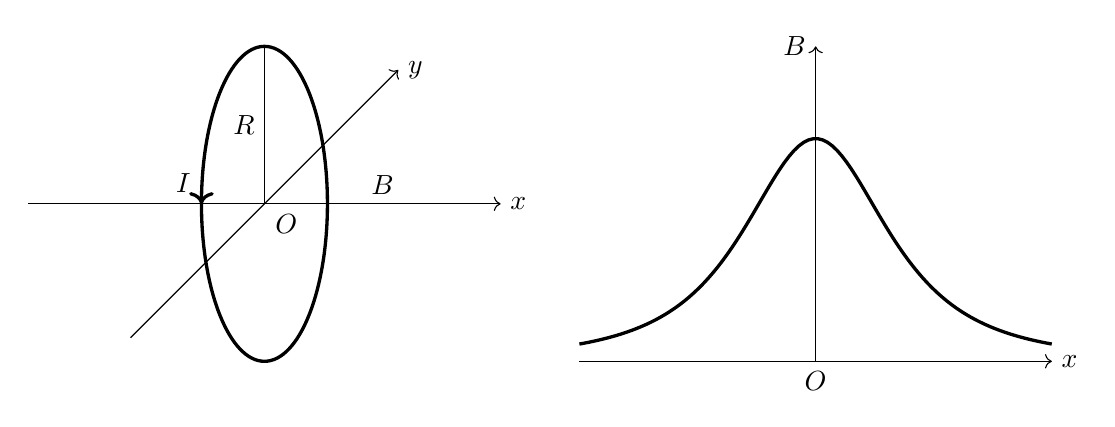
\begin{tikzpicture}
        \draw[very thick] (0,0)node[below right]{$ O $} ellipse (0.8 and 2);
        \draw[very thick,->] (-0.8,0.1)--(-0.8,0)node[above left]{$ I $};
        \draw[->] (-3,0)--(3,0)node[right]{$ x $};
        \draw (0,0)--node[left,midway]{$ R $}(0,2);
        \draw[->] (-1.7,-1.7)--(1.7,1.7)node[right]{$ y $};
        \node[above] at(1.5,0) {$ B $};
        
        \draw[->] (4,-2)--(10,-2)node[right]{$ x $};
        \draw[->] (7,-2)node[below]{$ O $}--(7,2)node[left]{$ B $};
        \draw[very thick, domain=4:10,samples=100] plot (\x,{16/(2*pow(2+pow(\x-7,2),1.5))-2});
    \end{tikzpicture}
    \caption{载流圆线圈轴向磁感应强度分布}
\end{figure}

在本实验中,圆线圈的参数取值如下:匝数 $N_0 = 400$ 匝,半径 $R = 105 \, \mathrm{mm}$。当频率 $f = 120 \, \mathrm{Hz}$,电流 $I = 60 \, \mathrm{mA}$\footnote{此部分实验所用 $I$ 均为有效值。},并且在圆心位置 $X = 0$ 时,可以利用圆线圈轴线上磁感应强度公式:
\[
B = \frac{\mu_0 N_0 I R^2}{2 (R^2 + X^2)^{3/2}}
\]
进行计算。 \par
在圆心处 $X = 0$ 时,公式可简化为:
\[
B = \frac{\mu_0 N_0 I}{2 R}
\]
将已知数据代入:
\[
B = \frac{(4\pi \times 10^{-7}) \times 400 \times (60 \times 10^{-3})}{2 \times (105 \times 10^{-3})}
\]
计算得单个圆线圈在圆心处的磁感应强度约为:
\[
B = 0.144 \, \mathrm{mT}.
\]

\subsubsection{亥姆霍兹线圈的磁感应强度}
所谓亥姆霍兹线圈,是指两组彼此平行且共轴(轴线重合)的圆线圈,并使两个线圈上流过相同方向的电流 $I$。根据理论证明,当两个线圈的中心间距 $a$ 等于线圈的半径 $R$ 时,这两个单线圈在轴线(两线圈圆心连线)上的磁场叠加后,在轴线中点附近较大的范围内可以形成一个均匀的磁场。下图形象地展示了这一均匀磁场形成的特性:
\begin{figure}[!h]
    \centering
    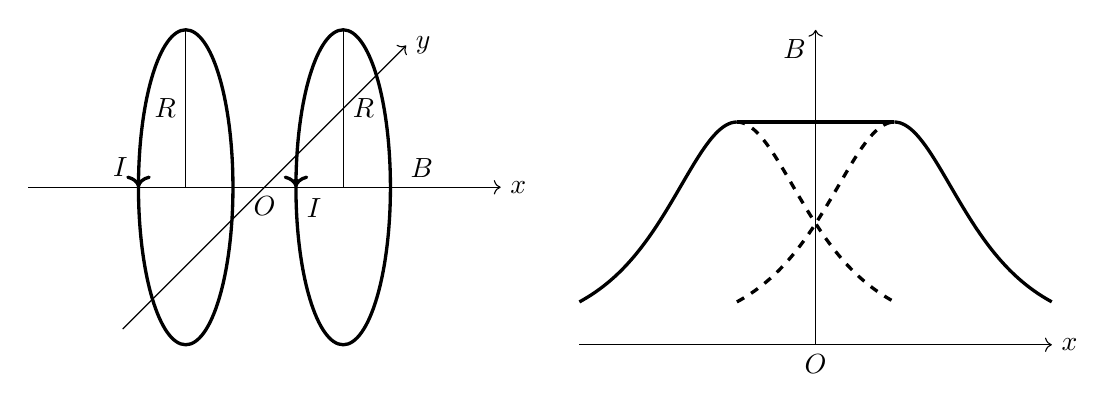
\begin{tikzpicture}
        \draw[very thick] (-1,0) ellipse (0.6 and 2);
        \draw[very thick] (1,0) ellipse (0.6 and 2);
        \draw[very thick,->] (-1.6,0.1)--(-1.6,0)node[above left]{$ I $};
        \draw[very thick,->] (0.4,0.1)--(0.4,0)node[below right]{$ I $};
        \draw[->] (-3,0)--(3,0)node[right]{$ x $};
        \draw[->] (-1.8,-1.8)--(1.8,1.8)node[right]{$ y $};
        \node[below] at(0,0) {$ O $};
        \draw (-1,0)--node[left,midway]{$ R $}(-1,2);
        \draw (1,0)--node[right,midway]{$ R $}(1,2);
        \node[above] at(2,0) {$ B $};
        
        \draw[->] (4,-2)--(10,-2)node[right]{$ x $};
        \draw[->] (7,-2)node[below]{$ O $}--(7,2)node[below left]{$ B $};
        \draw[very thick,domain=4:6,samples=100] plot (\x,{16/(2*pow(2+pow(\x-6,2),1.5))-2});
        \draw[very thick,dashed,domain=6:8,samples=100] plot (\x,{16/(2*pow(2+pow(\x-6,2),1.5))-2});
        \draw[very thick,dashed,domain=6:8,samples=100] plot (\x,{16/(2*pow(2+pow(\x-8,2),1.5))-2});
        \draw[very thick, domain=8:10,samples=100] plot (\x,{16/(2*pow(2+pow(\x-8,2),1.5))-2});
        \draw[very thick] (6,0.828)--(8,0.828);			
    \end{tikzpicture}
    \caption{亥姆霍兹线圈的磁感应强度分布}
\end{figure}

在亥姆霍兹线圈中,设轴线上某一点距离中心点 $O$ 的距离为 $z$,该点的磁感应强度 $B$ 可表示为:
\[
B = \frac{1}{2} \mu_0 N I R^2 \left\{ 
\left[
R^2 + \left( \frac{R}{2} + z \right)^2 
\right]^{-3/2} 
+ 
\left[
R^2 + \left( \frac{R}{2} - z \right)^2 
\right]^{-3/2}
\right\}
\]

当 $z = 0$ 时,即中心点 $O$ 处,根据公式计算,磁感应强度为:
\[
B = \frac{\mu_0 N_0 I}{2 R} \times \frac{16}{5^{3/2}}
\]

在本实验中,亥姆霍兹线圈的参数如下:匝数 $N_0 = 400$ 匝,半径 $R = 105 \, \mathrm{mm} = 0.105 \, \mathrm{m}$,频率 $f = 120 \, \mathrm{Hz}$,电流 $I = 60 \, \mathrm{mA} = 0.06 \, \mathrm{A}$。当 $z = 0$ 时,套用上述公式计算亥姆霍兹线圈的合成磁感应强度。

将已知数据代入:
\[
B = \frac{(4 \pi \times 10^{-7}) \times 400 \times 0.06}{2 \times 0.105} \times \frac{16}{5^{3/2}}
\]

计算得:
\[
B = 2.05 \, \mathrm{mT}.
\]

因此,在中心点 $O$ 处 ($z = 0$),亥姆霍兹线圈的合成磁感应强度为 $B = 2.05 \, \mathrm{mT}$。

\subsubsection{电磁感应法测磁感应强度}
由交流信号驱动的线圈会产生交变磁场,在任意时刻的磁感应强度瞬时值可以表示为:
\[
B = B_m \sin \omega t
\]
其中,$B_m$ 是磁感应强度的峰值,$\omega$ 为角频率。\par

若采用匝数为 $N$、截面积为 $S$、法线与磁场夹角为 $\theta$ 的探测线圈,其磁通量为:
\[
\Phi = N S B_m \cos \theta \sin \omega t
\]

根据法拉第电磁感应定律,其产生的感应电动势为磁通量对时间的负导数:
\[
\varepsilon = -\frac{d\Phi}{dt} = N S \omega B_m \cos \theta \cos \omega t = -\varepsilon_m \cos \omega t
\]
其中,$\varepsilon_m = N S \omega B_m \cos \theta$ 是感应电动势的峰值。\par

若使用数字式毫伏表测量该线圈的感应电动势,毫伏表的显示值 $U_{\max}$ 为电动势有效值 $\varepsilon_{\mathrm{rms}}$,即:
\[
U_{\max} = \frac{\varepsilon_m}{\sqrt{2}}
\]

由此可以反推出磁感应强度的峰值 $B_{\max}$:
\[
B_{\max} = \frac{\varepsilon_m}{N S \omega} = \frac{\sqrt{2} \, U_{\max}}{N S \omega}
\]

因此,通过测量线圈感应电动势 $U_{\max}$,结合匝数 $N$、截面积 $S$ 和角频率 $\omega$,即可计算磁感应强度的峰值 $B_{\max}$。

\section{实验内容}
\subsection{霍尔效应测量磁感应强度}
\subsubsection{正确连接电路}
\begin{enumerate}
    \item 将测试仪面板上的“$I_M$输入”,“$I_S$输出”和“$V_H$输入”三对接线柱分别与测试架上的相应三对接线柱连接。\par
    \item 将控制电源连接线的一端插入测试仪背面的控制电源输出插孔,另一端连接到测试架的控制电源输入插孔。\par
    \item 将测试仪的传感器接口与测试架上的传感器接口连接。\par
\end{enumerate}

\subsubsection{测量霍尔电压 $V_H$ 与工作电流 $I_S$ 的关系}
\begin{enumerate}
    \item 设定 $I_M = 0$ 的条件下,将霍尔效应试验仪调零,并将霍尔元件片置于电磁铁的中心位置。\par
    \item 将励磁电流 $I_H = 200 \, \mathrm{mA}$ 和工作电流 $I_S = 0.5 \, \mathrm{mA}$,调节励磁电流 $I_M$ 和工作电流 $I_S$ 的方向,测量相应的电压值 $V_1$、$V_2$、$V_3$、$V_4$,并记录数据。\par
    \item 每次将工作电流 $I_S$ 增加 $0.50 \, \mathrm{mA}$,测量并记录电压值 $V_1$、$V_2$、$V_3$、$V_4$。\par
\end{enumerate}

\subsubsection{测量霍尔电压 $V_H$ 和磁感应强度 $B$ 与励磁电流 $I_M$ 的关系}
\begin{enumerate}
    \item 将 $I_M$ 和 $I_S$ 调零后,设定工作电流 $I_S = 1.00 \, \mathrm{mA}$。调节励磁电流 $I_M$ 和工作电流 $I_S$ 的方向,测量相应的电压值 $V_1$、$V_2$、$V_3$、$V_4$,并记录数据。\par
    \item 每次将励磁电流 $I_M$ 增加 $50 \, \mathrm{mA}$,测量并记录电压值 $V_1$、$V_2$、$V_3$、$V_4$ 和磁感应强度值 $B_1$、$B_2$、$B_3$、$B_4$。\par
\end{enumerate}

\subsubsection{计算霍尔元件的霍尔灵敏度}
根据公式 $V_H = K_H I_S B$,可以得出霍尔灵敏度的计算公式:
\[
K_H = \frac{V_H}{I_S B}
\]
选取实验中测得的几组数据,计算相应的 $K_H$,并与实验仪器上标注的霍尔灵敏度 $K_H$ 进行比较,计算相对误差。

\subsubsection{测量电磁铁磁场沿水平方向分布}
\begin{enumerate}
    \item 在励磁电流 $I_M = 0$ 的条件下,将毫特计调零。\par
    \item 设定励磁电流 $I_M = 200 \, \mathrm{mA}$,调节移动尺的位置,每间隔 $2 \, \mathrm{mm}$ 记录一次毫特计的读数值。\par
\end{enumerate}

\subsubsection{用交流霍尔电流测量磁场}
\begin{enumerate}
    \item 将霍尔效应试验仪调零,并将霍尔元件重新移动到电磁铁的中心位置。\par
    \item 修改接线方式,使用信号发生器代替直流稳压电源。\par
    \item 调节信号发生器的频率至 $f = 500 \, \mathrm{Hz}$,并调节输出电压以保证交流工作电流 $I_S = 1 \, \mathrm{mA}$。\par
    \item 分别测量在 $I_M = 10 \, \mathrm{mA}$,$I_M = 100 \, \mathrm{mA}$,$I_M = 150 \, \mathrm{mA}$ 和 $I_M = 200 \, \mathrm{mA}$ 时的霍尔电压 $V_{H-\mathrm{AC}}$。\par
\end{enumerate}
\subsection{亥姆霍兹线圈的磁感应强度测量}
\subsubsection{测量圆电流线圈轴线上磁感应强度分布}
\begin{enumerate}
    \item 正确连接电路,使单个线圈通以电流。\par
    \item 将磁感应强度实验仪调零。\par
    \item 调节电位器,将频率设为 $f = 120 \, \mathrm{Hz}$,并设定励磁电流的有效值为 $I = 60 \, \mathrm{mA}$。\par
    \item 以圆电流线圈的中心为坐标原点,每隔 $5 \, \mathrm{mm}$ 测量一次 $U_{\max}$ 的值,记录实验数据。\par
\end{enumerate}

\subsubsection{测量亥姆霍兹线圈轴线上磁感应强度分布}
\begin{enumerate}
    \item 正确连接电路,使两个线圈通以大小相等的电流。\par
    \item 在励磁电流为零的情况下,将磁感应强度实验仪调零。\par
    \item 调节电位器,将频率设为 $f = 120 \, \mathrm{Hz}$,并设定励磁电流的有效值为 $I_M = 60 \, \mathrm{mA}$。\par
    \item 以亥姆霍兹线圈的中心为坐标原点,每隔 $5 \, \mathrm{mm}$ 测量一次磁感应强度 $U_{\max}$ 的值,记录实验数据。\par
\end{enumerate}

\subsubsection{测量亥姆霍兹线圈磁场径向分布}
\begin{enumerate}
    \item 固定探测线圈与圆电流线圈轴线的夹角为 $0^{\circ}$,并将探测线圈的位置调到亥姆霍兹线圈的中心处。\par
    \item 转动径向移动手轮,每隔 $5 \, \mathrm{mm}$ 记录一次 $U_{\max}$ 的值。\par
\end{enumerate}

\subsubsection{测量线圈转角与感应电压的关系}
\begin{enumerate}
    \item 将探测线圈移动到亥姆霍兹线圈的中心位置。\par
    \item 从转角 $0^{\circ}$ 开始,每改变 $10^{\circ}$ 记录一次实验数据,直到转角为 $180^{\circ}$。\par
\end{enumerate}

\subsubsection{探究励磁电流频率对磁感应强度的影响}
\begin{enumerate}
    \item 将探测线圈的角度设置为 $0^{\circ}$,并保持其位置在亥姆霍兹线圈中心点。\par
    \item 调节电流的频率,在 $20 \sim 120 \, \mathrm{Hz}$ 的范围内,每次改变 $10 \, \mathrm{Hz}$,并保持$I=60mA$不变,记录对应的 $U_{\max}$ 数据。\par
\end{enumerate}

\section{实验数据记录}
    \subsection{霍尔电压$V_H$与工作电流$I_S$的关系数据记录}
    \newpage
        \begin{table}[!h]
            \centering
            \begin{tabular}{|l|l|l|l|l|l|}
            \hline
                \multicolumn{6}{|c|}{$V_H$-$I_S$($I_M$=200mA)}\\ \hline
                \multirow{2}*{$I_S$(mA)} & $V_1$(mV) & $V_2$(mV) & $V_3$(mV) & $V_4$(mV) & \multirow{2}*{$V_H$} \\ \cline{2-5}
                ~ & +$I_M$+$I_S$ & +$I_M$-$I_S$ & -$I_M$-$I_S$ & -$I_M$+$I_S$ & ~ \\ \hline
                0 & 0.0 & 0.0 & 0.0 & 0.0 & 0.0 \\ \hline
                0.50 & 26.8 & -26.8 & 27.6 & -27.6 & 27.2 \\ \hline
                1.00 & 53.4 & -53.4 & 54.9 & -54.9 & 54.2 \\ \hline
                1.50 & 80.2 & -80.2 & 82.5 & -82.4 & 81.3 \\ \hline
                2.00 & 107.1 & -107.0 & 110.1 & -110.0 & 108.6 \\ \hline
                2.50 & 133.4 & -133.4 & 137.2 & -137.1 & 135.3 \\ \hline
                3.00 & 160.2 & -160.1 & 164.8 & -164.6 & 162.4\\ \hline
            \end{tabular}
        \end{table}
    \subsection{霍尔电压$V_H$与励磁电流$I_M$的关系数据记录}
        \begin{table}[!h]
            \centering
            \begin{tabular}{|l|l|l|l|l|l|}
            \hline
                \multicolumn{6}{|c|}{$V_H-I_M(I_S=1.00mA)$}\\ \hline
                \multirow{2}*{$I_M$(mA)} & $V_1$(mV) & $V_2$(mV) & $V_3$(mV) & $V_4$(mV) & \multirow{2}*{$V_H$} \\ \cline{2-5}
                ~ & $+I_M+I_S$ & $I_M-I_S$ & $-I_M-I_S$ & $-I_M+I_S$ & ~ \\ \hline
                0 & 0 & 0 & 0 & 0 & 0 \\ \hline
                50 & 13.0 & -13.0 & 14.6 & -14.6 & 13.8 \\ \hline
                100 & 26.3 & -26.3 & 28.0 & -28.0 & 27.2 \\ \hline
                150 & 40.2 & -40.2 & 41.8 & -41.8 & 41.0 \\ \hline
                200 & 53.8 & -53.8 & 55.4 & -55.4 & 54.6 \\ \hline
                250 & 67.4 & -67.4 & 69.0 & -69.0 & 68.2 \\ \hline
                300 & 80.8 & -80.8 & 82.5 & -82.4 & 81.6 \\ \hline
            \end{tabular}
        \end{table}

    \subsection{磁感应强度B与励磁电流$I_M$的关系数据记录}
        \begin{table}[!h]
            \centering
            \begin{tabular}{|l|l|l|l|l|l|}
            \hline
                \multicolumn{6}{|c|}{$B-I_M(I_S=1.00mA)$}  \\ \hline
                \multirow{2}*{$I_M$(mA)} & $B_1(mT)$ & $B_2(mT)$ & $B_3(mT)$ & $B_4(mT)$ & \multirow{2}*{B} \\ \cline{2-5}
                ~ & $+I_M+I_S$ & $+I_M-I_S$ & $-I_M-I_S$ & $-I_M+I_S$ & ~ \\ \hline
                0 & 0 & 0 & 0 & 0 & 0 \\ \hline
                50 & 38.6 & 38.5 & -38.1 & -38.1 & 38.3 \\ \hline
                100 & 75.2 & 75.2 & -75.1 & -75.1 & 75.2 \\ \hline
                150 & 113.3 & 113.3 & -113.0 & -113.0 & 113.2\\ \hline
                200 & 150.7 & 150.7 & -150.5 & -150.4 & 150.6 \\ \hline
                250 & 188.3 & 188.3 & -188.1 & -188.1 & 188.2\\ \hline
                300 & 225.1 & 225.1 & -225.0 & -225.0 & 225.1 \\ \hline
            \end{tabular}
        \end{table}
    
    \subsection{电磁铁磁场沿水平方向分布数据记录}
        \begin{table}[!h]
            \centering
            \begin{tabular}{|l|l|l|l|l|l|l|l|l|}
            \hline
                \multicolumn{9}{|c|}{电磁铁磁场沿水平方向分布数据   ($I_M$=200mA)} \\ \hline
                X/mm & 42 & 40 & 38 & 36 & 34 & 32 & 30 & 28\\ \hline
                B/mT  & 35.8 & 61.0 & 120.7 & 148.9 & 149.8 & 149.9 & 150.0 & 149.9\\ \hline
                X/mm  & 26 & 24 & 22 & 20 & 18 & 16 &  & \\ \hline
                B/mT & 149.7 & 149.8 & 149.8 & 149.8 & 149.8 & 149.7 & & \\ \hline
            \end{tabular}
        \end{table}

    \subsection{AC模式霍尔效应测量磁场数据记录}
        \begin{table}[!h]
            \centering
            \begin{tabular}{|l|l|l|l|l|l|l|l|l|}
            \hline
                \multicolumn{8}{|c|}{AC模式霍尔效应测量磁场($I_{S-AC}$=1mA)} \\ \hline
                $I_M$(mA) & 50 & 75 & 100 & 125 & 150 & 175 & 200 \\ \hline
                B/mT & 37.8 & 56.2 & 74.9 & 93.8 & 112.5 & 130.9 & 150.2 \\ \hline
                $V_{H-AC}$/mV & 15.03 & 21.77 & 28.67 & 35.57 & 42.43 & 49.19 & 56.22 \\ \hline
            \end{tabular}
        \end{table}
    
        \subsection{圆电流线圈轴线上磁场分布测量数据记录}
        \begin{table}[!h]
            \centering
            \begin{tabular}{|l|c|c|c|c|c|c|c|c|c|c|c|}
            \hline
                \multicolumn{12}{|c|}{圆电流线圈轴线上磁场分布测量数据记录}  \\ \hline
                轴向距离 $X$ (mm) & -25 & -20 & -15 & -10 & -5 & 0 & 5 & 10 & 15 & 20 & 25 \\ \hline
                $U_{\text{max}}$ (mV) & 5.40 & 5.54 & 5.71 & 5.76 & 5.91 & 5.93 & 5.91 & 5.84 & 5.78 & 5.61 & 5.51 \\ \hline
                测量值 $B$ (mT) & 0.132 & 0.135 & 0.139 & 0.141 & 0.145 & 0.143 & 0.144 & 0.142 & 0.141 & 0.137 & 0.134 \\ \hline
                计算值 $B$ (mT) & 0.132 & 0.136 & 0.139 & 0.142 & 0.143 & 0.144 & 0.143 & 0.142 & 0.139 & 0.136 & 0.132 \\ \hline
                \multicolumn{12}{|l|}{\( f = 120\,\text{Hz},\quad I = 60\,\text{mA},\quad N_0 = 400,\quad R = 105\,\text{mm} \)} \\ \hline
            \end{tabular}
        \end{table}

    \subsection{亥姆霍兹线圈轴线上磁场分布测量数据记录}
        \begin{table}[!h]
            \centering
            \begin{tabular}{|l|l|l|l|l|l|l|l|l|l|l|l|}
            \hline
                \multicolumn{12}{|c|}{亥姆霍兹线圈轴线上磁场分布测量数据记录}  \\ \hline
                轴向距离X(mm) & -25 & -20 & -15 & -10 & -5 & 0 & 5 & 10 & 15 & 20 & 25 \\ \hline
                $U_{max}$(mV) & 7.93 & 7.95 & 7.96 & 7.96 & 7.96 & 7.96 & 7.96 & 7.96 & 7.96 & 7.94 & 7.93 \\ \hline
                测量值B(mT) & 0.193 & 0.194 & 0.194 & 0.194 & 0.194 & 0.194 & 0.194 & 0.194 & 0.194 & 0.194 & 0.193 \\ \hline
                \multicolumn{12}{|l|}{f=120Hz,I=60mA} \\ \hline
            \end{tabular}
        \end{table}
    
    \subsection{亥姆霍兹线圈磁场径向分布测量数据记录}
        \begin{table}[!h]
            \centering
            \begin{tabular}{|l|l|l|l|l|l|l|l|l|l|l|l|}
            \hline
                \multicolumn{12}{|c|}{亥姆霍兹线圈磁场径向分布测量数据记录} \\ \hline
                径向距离X(mm) & -25 & -20 & -15 & -10 & -5 & 0 & 5 & 10 & 15 & 20 & 25 \\ \hline
                $U_{max}$(mV) & 8.61 & 8.62 & 8.63 & 8.63 & 8.63 & 8.64 & 8.63 & 8.62 & 8.62 & 8.62 & 8.61 \\ \hline
                测量值B(mT) & 0.210 & 0.210 & 0.210 & 0.210 & 0.210 & 0.211 & 0.210 & 0.210 & 0.210 & 0.210 & 0.210 \\ \hline
                \multicolumn{12}{|l|}{f=120Hz,I=60A} \\ \hline
            \end{tabular}
        \end{table}

        \subsection{探测线圈转角与感应电压数据记录}
        \newpage
        \begin{table}[!h]
            \centering
            \begin{tabular}{|l|l|l|l|l|l|l|l|l|l|l|}
            \hline
                \multicolumn{11}{|c|}{探测线圈转角与感应电压测量数据记录} \\ \hline
                探测线圈转角$\theta$ & 0 & 10 & 20 & 30 & 40 & 50 & 60 & 70 & 80 & 90 \\ \hline
                U(mV) & 8.64 & 8.53 & 8.14 & 7.64 & 6.73 & 5.73 & 4.48 & 3.15 & 1.64 & 0.12 \\ \hline
                计算值(mV) & 8.64 & 8.51& 8.12 & 7.48 & 6.62 & 5.55 & 4.32 & 2.96 & 1.50 & 0.00 \\ \hline
                探测线圈转角$\theta$ & 100 & 110 & 120 & 130 & 140 & 150 & 160 & 170 & 180 & 190 \\ \hline
                U(mV) & 1.47 & 2.93 & 4.38 & 5.62 & 6.73 & 7.57 & 8.21 & 8.62 & 8.73 & 8.57\\ \hline
                计算值(mV) & 1.50 & 2.96 &4.32& 5.55 & 6.62 & 7.48 & 8.12 & 8.51 & 8.64 & 8.51 \\ \hline
                探测线圈转角$\theta$ & 200 & 210 & 220 & 230 & 240 & 250 & 260 & 270 & 280 & 290 \\ \hline
                U(mV) & 8.13 & 7.48 & 6.56 & 5.35 & 4.18 & 2.78 & 1.28 & 0.20 & 1.76 & 3.14\\ \hline
                计算值(mV) & 8.12 & 7.48 & 6.62 & 5.55 & 4.32 & 2.96 & 1.50 & 0.00 & 1.50 &2.96\\ \hline
                探测线圈转角$\theta$ & 300 & 310 & 320 & 330 & 340 & 350 & 360 & ~ & ~& ~ \\ \hline
                U(mV) & 4.47 & 5.62 & 6.68 & 7.54 & 8.06 & 8.49 & 8.64 & ~ & ~ & ~\\ \hline
                计算值(mV) & 4.32 & 5.55 & 6.62 & 7.48 & 8.12 & 8.51 & 8.64 & ~ & ~ & ~ \\ \hline
            \end{tabular}
        \end{table}

    \subsection{励磁电流频率对磁场强度的影响}
        \begin{table}[!h]
            \centering
            \begin{tabular}{|l|l|l|l|l|l|l|l|l|l|l|l|}
            \hline
                \multicolumn{12}{|c|}{励磁电流频率对磁场强度的影响}  \\ \hline
                励磁电流频率f(Hz) & 20 & 30 & 40 & 50 & 60 & 70 & 80 & 90 & 100 & 110 & 120 \\ \hline
                $U_{max}$(mV) & 1.43 & 2.15 & 2.88 & 3.60 & 4.31 & 5.02 & 5.74 & 6.46 & 7.19 & 7.92 & 8.63 \\ \hline
                测量值(mT) & 0.209 & 0.210 & 0.211 & 0.211 & 0.210 & 0.210 & 0.210 & 0.210 & 0.210 & 0.211 & 0.210 \\ \hline
                \multicolumn{12}{|l|}{I=60mA(注意:始终保持在60mA)} \\ \hline
            \end{tabular}
        \end{table}
    
\section{数据处理及结果}
\subsection{霍尔电压$V_H$与工作电流$I_S$的关系}
    \begin{figure}[!h]
        \centering
        \includegraphics[scale=0.8]{output1.png}
        \caption{霍尔电压$V_H$与工作电流$I_S$的关系图}
    \end{figure}
    利用python的scipy库进行线性拟合,得到如上图所示的拟合直线图,发现实验数据呈现出很好的线性关系,且纵截距为0.09,
    在实验误差允许范围内可近似为0,不为0的原因可能是埃延霍森效应导致的。

\subsection{霍尔电压$V_H$与磁感应强度$B$的关系与霍尔灵敏度}
    \begin{figure}[!h]
        \centering
        \includegraphics[scale=0.8]{output2.png}
        \caption{霍尔电压$V_H$与磁感应强度$B$的关系图}
    \end{figure}
    利用python的scipy库进行线性拟合,得到如上图所示的拟合直线图,发现实验数据呈现出很好的线性关系,且纵截距为-0.05,
    在实验误差允许范围内可近似为0,不为0的原因可能是埃延霍森效应导致的。
    
    由图可知$K_{H-B}=0.36$,根据公式$K_H = \frac{V_H}{I_S B}=\frac{K_{H-B}}{I_S}$得到霍尔灵敏度$K_H = 360.0\, \mathrm{mV/(mA\cdot T)}$。

    下面计算不确定度,根据最小二乘法斜率相对不确定度的计算公式:
    \[
    \frac{u(x)}{x} = \sqrt{\frac{\frac{1}{R^2} - 1}{N - 2}}
    \]
    
    我们可以计算霍尔电压 $V_H$ 与励磁电流 $I_M$ 的斜率不确定度为:
    \[
    \frac{u(V_H / I_M)}{V_H / I_M} = 1.0 \times 10^{-2}
    \]
    
    同时,磁感应强度 $B$ 与励磁电流 $I_M$ 的斜率不确定度为:
    \[
    \frac{u(B / I_M)}{B / I_M} = 3.5 \times 10^{-3}
    \]
    
    根据不确定度合成公式,得到霍尔灵敏度 $K_H$ 的相对不确定度为:
    \[
    \frac{u(K_H)}{K_H} = 1.2 \times 10^{-2}
    \]
    
    由此可得,霍尔灵敏度 $K_H$ 的绝对不确定度为:
    \[
    u(K_H) = 4.32 \, \mathrm{V/(A \cdot T)}
    \]
    
    因此,霍尔灵敏度 $K_H$ 的最终测量结果为:
    \[
    K_H = (360.0 \pm 4.32) \, \mathrm{V/(A \cdot T)}
    \]

\subsection{磁感应强度$B$与励磁电流$I_M$的关系}
    \begin{figure}[!h]
        \centering
        \includegraphics[scale=0.8]{output3.png}
        \caption{磁感应强度$B$与励磁电流$I_M$的关系图}
    \end{figure}
    利用python的scipy库进行线性拟合,得到如上图所示的拟合直线图,发现实验数据呈现出很好的线性关系,且纵截距为0.39,
    相比于上面两组关系,纵截距较大,说明励磁电流为0时仍存在一定磁感应强度。这可能是因为本组关系数据在零点处霍尔电流数量级远大于上一组数据,根据埃廷豪森效应温差电动势$V_E\propto{IB}$的关系,
    埃廷豪森效应的影响较前两组关系图更大,因而误差也相应增大。

\subsection{电磁铁磁感应强度沿水平方向分布}
    \begin{figure}[!h]
        \centering
        \includegraphics[scale=0.6]{output4.png}
        \caption{电磁铁磁感应强度沿水平方向分布$(I_M=200mA)$}
    \end{figure}
    由图像可以看出,在一定范围内电磁铁的磁感应强度基本保持不变,而在$X>36cm$后磁感应强度迅速减小,这基本符合理论预期。

\subsection{AC模式霍尔效应测量磁场}
\begin{figure}[!h]
    \centering
    \includegraphics[scale=0.8]{output5.png}
    \caption{磁感应强度$B$与交流霍尔电压$V_{H-AC}$的关系图}
\end{figure}
继续利用python的scipy库进行线性拟合,得到如上图所示的拟合直线图。从实验图像中可以看出,霍尔电压 $V_H$ 与磁感应强度 $B$ 呈现出高度线性关系,且线性相关性非常强。然而,图像中的截距与 0 存在较大的偏差。 \par

根据对霍尔元件副效应的分析,诸如埃廷豪森效应、托伦斯效应和里纪-杜勒克效应的影响都应该被显著削弱。这是因为温差的建立需要一定的弛豫时间,而交流电的应用会干扰温差的积累过程,使得温差无法完全建立,从而减小了温差相关副效应对测量结果的影响。 \par

根据理论公式:
\[
V_H = K_H I_S B
\]
可以得到霍尔元件的灵敏度为:
\[
K_H = 364.73 \, \mathrm{mV/(mA \cdot T)}
\]

此外,根据之前的最小二乘法不确定度公式,可以看出测量值的不确定度较小,因而测量结果具有较高的可靠性。这表明应用交流电可以更有效地降低副效应对测量的影响,从而提高测量的准确性。
\subsection{圆电流线圈轴线上磁感应强度分布}
\begin{figure}[!h]
    \centering
    \includegraphics[scale=0.8]{output6.png}
    \caption{圆电流线圈轴线上的磁感应强度分布}
\end{figure}
利用python的scipy库进行插值计算并生成较为平滑的磁场分布图。
对图像中磁感应强度随轴向距离的变化进行分析可以得出,圆线圈的磁感应强度随着位置的增大呈现出先上升的趋势,在 $X = 0$ 处达到极大值,随后开始下降。此外,图像呈现出关于 $X = 0$ 点的轴对称性。 \par

通过对比测量值与计算值,可以发现测量值与理论计算值较为接近(注意分度值较小,从而这一结果较为准确),且测量值较好地呈现出关于 $X = 0$ 轴的对称性。
此外,可以注意到,每组数据中理论值与测量值相差的数量级接近,大约为 $10^{-5} \, \mathrm{T}$。这一数量级恰与地磁场的典型大小接近,因此可以推测,理论值与计算值之间的误差可能还受到实验环境中地磁场的影响。

\subsection{亥姆霍兹线圈轴线上磁感应强度分布}
\begin{figure}[!h]
    \centering
    \includegraphics[scale=0.8]{output7.png}
    \caption{亥姆霍兹线圈轴线上的磁感应强度分布}
\end{figure}
从图像中可以观察到,磁感应强度在轴线上近似恒定,这与理论预期相符。然而,数据中仍然存在一定程度的波动。 \par

这种波动现象可以归因于实验条件中的实际因素。由于亥姆霍兹线圈中通入的是交变电流,导致实验过程中测量的读数经常会在两个临近值之间波动。在实际记录读数时,通常只选择其中一个值进行记录。因此,该部分误差的主要来源为读数误差。
\subsection{亥姆霍兹线圈磁感应强度径向分布}
\begin{figure}[!h]
    \centering
    \includegraphics[scale=0.8]{output8.png}
    \caption{亥姆霍兹线圈径向磁感应强度分布}
\end{figure}
从图像中可以观察到,在亥姆霍兹线圈 $X = 0$ 处,磁感应强度沿径向近似保持不变,这与理论预言一致。然而,实验数据中仍然存在一些波动。 \par

这种误差与上一个图表中所描述的情况一致,主要原因在于测量交变电流电压时,读数在两个临近值之间发生波动。由于实际读数通常选择其中一个值进行记录,因此这一波动成为导致实验数据误差的主要来源。
\newpage

\subsection{探测线圈转角与感应电压的关系}
\begin{figure}[!h]
    \centering
    \includegraphics[scale=0.8]{output9.png}
    \caption{亥姆霍兹线圈探测线圈转角与感应电压的关系}
\end{figure}
从图像中可以看出,感应电压随着转角的变化呈现出先增大后减小的规律。当转角 $\theta = 90^\circ$ 时,感应电压达到极小值。随后,随着转角继续增大,感应电压再次增大。此外,图像整体呈现出关于中心轴的对称性,这一趋势与理论预期相符,并且理论曲线与实际测量曲线非常接近。\par

然而注意到在 $\theta = 90^\circ$ 时,测量值并不严格等于零,这表明存在偏差。
这种偏差可能的主要来源是线圈绕制过程中的不均匀性引入了误差,从而导致测量结果与理论值出现微小的偏移。

\subsection{励磁电流频率对磁场强度的影响}
\begin{figure}[!h]
    \centering
    \includegraphics[scale=0.8]{output10.png}
    \caption{励磁电流频率对磁场强度的影响}
\end{figure}
从图像中可以看出,励磁电流的频率对磁感应强度几乎没有影响,这与理论预言一致。然而,磁场强度的测量结果中仍然存在一些误差。\par

这些误差可能的来源包括以下几点:
\begin{itemize}
    \item \textbf{读数波动}:由于交变电流带来的不稳定性,测量过程中的读数经常会在两个临近值之间波动,导致记录的读数存在误差。
    \item \textbf{励磁电流调节误差}:在实际测量中,调节励磁电流频率的同时,励磁电流强度也会发生变化。因此,需要在调节频率的同时手动调节励磁电流强度以保持在 $60 \, \mathrm{mA}$ 不变,受到仪器测量精度影响励磁电流可能会发生微小变化,进一步增加测量误差。
\end{itemize}

\section{讲义思考题}
\subsection{霍尔效应测量磁感应强度}
        \subsubsection{分析本实验主要误差来源,计算磁感应强度B的合成不确定度(分别取$I_M=0.2A,I_S=1mA$)}
        \textbf{误差来源分析:} \par
实验中的主要误差来源包括以下几点:
\begin{enumerate}
    \item \textbf{埃廷豪森效应的影响}:埃廷豪森效应无法被完全消除,一直是误差的重要来源。\par
    \item \textbf{实验仪器本身的误差}:实验中所用仪器存在一定的系统误差,例如霍尔高斯计、毫伏表等的精度限制。\par
    \item \textbf{读数误差}:由于测量过程中读数不稳定,波动导致读数误差。\par
    \item \textbf{地磁场的影响}:地磁场对实验环境中的磁场测量产生了额外的干扰。\par
\end{enumerate}

\textbf{不确定度计算:} \par
当 $I_M = 200 \, \mathrm{mA}$,$I_S = 1 \, \mathrm{mA}$ 时,实验数据给出 $V_H = 59.4 \, \mathrm{mV}$,$B = 144.9 \, \mathrm{mT}$。\par

根据磁感应强度公式:
\[
B = \frac{V_H}{{K_H I_S}}
\]

以及不确定度的传递规则,不确定度的相对值可以表示为:
\[
\frac{u(B)}{B} = \sqrt{ 
\left( \frac{u(V_H)}{V_H} \right)^2 + 
\left( \frac{u(K_H)}{K_H} \right)^2 + 
\left( \frac{u(I_S)}{I_S} \right)^2 
}
\]

根据实验计算及仪器参数:
\begin{itemize}
    \item $\frac{u(V_H)}{V_H} = 7.15 \times 10^{-4}$,
    \item $\frac{u(K_H)}{K_H} = 1.20 \times 10^{-2}$,
    \item $\frac{u(I_S)}{I_S} = 0.01$。
\end{itemize}

将上述值代入公式:
\[
\frac{u(B)}{B} = \sqrt{ 
\left( 7.15 \times 10^{-4} \right)^2 +
\left( 1.20 \times 10^{-2} \right)^2 + 
\left( 0.01 \right)^2 
}
\]

计算得:
\[
\frac{u(B)}{B} = 1.01 \times 10^{-2}.
\]

因此,磁感应强度的不确定度为:
\[
u(B) = B \cdot \frac{u(B)}{B} = 144.9 \, \mathrm{mT} \times 1.01 \times 10^{-2} = 1.46 \, \mathrm{mT}.
\]

最终磁感应强度的结果可以表示为:
\[
B = \left( 144.9 \pm 1.46 \right) \, \mathrm{mT}.
\]

\subsubsection{以简图示意,用霍尔效应判断霍尔片上磁感应强度的方向}
不妨将霍尔元件简化为一个长方体,其几何结构的示意图如下:
\begin{figure}[!h]
    \centering
    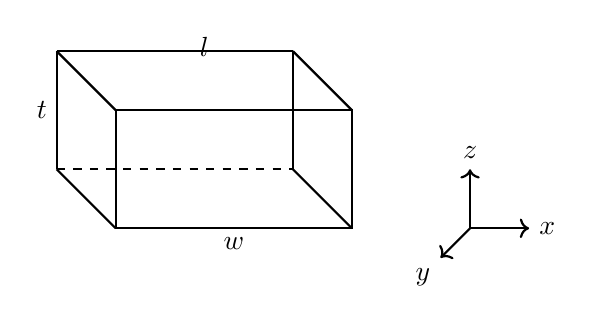
\begin{tikzpicture}[scale=1.5]
        % Draw the 3D rectangle (parallelepiped)
        % Front face
        \draw[thick] (0,0) rectangle (2,1);
        
        % Top face
        \draw[thick] (0,1) -- (-0.5,1.5);
        \draw[thick] (2,1) -- (1.5,1.5);
        \draw[thick] (-0.5,1.5) -- (1.5,1.5);
        
        % Right face
        \draw[thick] (2,0) -- (1.5,0.5);
        \draw[thick] (1.5,0.5) -- (1.5,1.5);
        
        % Connecting lines for 3D effect
        \draw[thick] (0,0) -- (-0.5,0.5);
        \draw[thick] (-0.5,0.5) -- (-0.5,1.5);
        \draw[thick, dashed] (-0.5,0.5) -- (1.5,0.5);
        
        % Labels
        \node[below] at (1,0) {$w$}; % width
        \node[left] at (-0.5,1) {$t$}; % thickness
        \node[above] at (0.75,1.375) {$l$}; % length
        
        % Coordinates axes
        \draw[->, thick] (3,0) -- (3.5,0) node[right] {$x$};
        \draw[->, thick] (3,0) -- (3,0.5) node[above] {$z$};
        \draw[->, thick] (3,0) -- (2.75,-0.25) node[below left] {$y$};
    \end{tikzpicture}
    \caption{长方体霍尔元件的示意图}
    \label{fig:Hall_Rectangular}
\end{figure}

将电流与y方向垂直的两个面之间,由外部电路的接法可以确定电流的流动方向。同时,可以通过测量与x方向垂直的两个面上的电势差,用电压表判断霍尔电压的方向。 \par

针对霍尔元件,我们有以下分析:
\begin{itemize}
    \item 若霍尔元件为 \textbf{P型} 半导体,其载流子为正电荷。正电荷的运动方向与外加电流的方向一致; \par
    \item 若霍尔元件为 \textbf{N型} 半导体,其载流子为负电荷。负电荷的运动方向与外加电流方向相反。
\end{itemize}

当电流稳定后,载流子受力达到平衡状态,即洛伦兹力与霍尔电压作用下的电场力相平衡。此时:
\begin{itemize}
    \item 洛伦兹力的方向与电场力方向相反;
    \item 电场力的方向可通过 $ADHE$ 面与 $BCGF$ 面的电势差正负,结合载流子的电荷性质推断。
\end{itemize}

已知洛伦兹力的方向与载流子的运动方向相关,因此可以通过矢量关系分析以下因素:
\begin{enumerate}
    \item \textbf{载流子运动方向}:由外加电流的流动方向结合载流子电性确定;
    \item \textbf{洛伦兹力方向}:由载流子的运动方向和磁场方向推导,通过右手定则或左手定则判断;
    \item \textbf{电场方向}:与x方向垂直的两个面的电势差正负确定;
    \item \textbf{磁场方向}:根据载流子受力平衡关系,通过矢量合成确定磁场的方向。
\end{enumerate}

\subsubsection{如何测量交变磁场,写出主要步骤}
为了研究交变磁场中霍尔元件的响应行为,可以采取以下实验方案: \par

\begin{enumerate}
    \item \textbf{利用霍尔元件观察交变磁场中的响应} \par
    将霍尔元件置于交变磁场中,并将霍尔电压连接到示波器上。通过观察示波器上的波形,可以直观展示霍尔元件在交变磁场中的响应行为,同时可以对波形的特征参数(如频率、幅值等)进行测量与分析。 \par

    \item \textbf{利用探测线圈测量交变磁场的磁感应强度} \par
    将探测线圈置于交变磁场中,并将线圈的两端连接至示波器:
    \begin{itemize}
        \item 转动探测线圈,找到电动势的峰值最大处,此时线圈的法向方向与磁场变化方向一致;
        \item 使用示波器记录感生电动势的波形,已知探测线圈的匝数 $N$ 和截面积 $S$,利用感生电动势公式:
        \[
        E = N S \frac{\dd B}{\dd t},
        \]
        可从波形曲线对感生电动势进行积分,从而计算得到交变磁场中磁感应强度 $B$ 随时间的变化关系:
        \[
        B(t) = \frac{1}{N S} \int E(t) \, \dd t.
        \]
    \end{itemize}
\end{enumerate}

通过以上方法,可以分别利用霍尔元件和探测线圈,清晰展示并分析交变磁场中磁感应强度的时变特性。

\subsection{亥姆霍兹线圈的磁感应强度测量}
\subsubsection{单线圈轴线上磁感应强度的分布规律如何?亥姆霍兹线圈是怎样组成的?其基本条件有哪些?它的磁感应强度分布特点怎样?}
1. 对于一个单个圆线圈,其半径为 $R$,匝数为 $N$,通入电流 $I$。在线圈中心轴线上距离中心为 $X$ 的位置处,其磁感应强度为:
\[
B = \frac{{\mu_0 N I R^2}}{{2 (R^2 + X^2)^{3/2}}},
\]
其中,$\mu_0$ 是真空磁导率。 \par

2. 亥姆霍兹线圈由两组平行且共轴、相同的载流圆线圈组成。两个线圈的中心间距等于线圈的直径,且两个线圈通有同向且大小相同的电流。 \par

3. 在亥姆霍兹线圈的轴线上,并且在两个线圈附近的区域内,磁场的分布非常均匀。亥姆霍兹线圈的磁感应强度 $B$ 表达式为:
\[
B = \frac{{\mu_0 N I R^2}}{2} \left\{
\frac{1}{{\left[R^2 + \left(\frac{R}{2} + X\right)^2\right]^{3/2}}} + 
\frac{1}{{\left[R^2 + \left(\frac{R}{2} - X\right)^2\right]^{3/2}}}
\right\}.
\]
对上述表达式在 $X = 0$ 点进行泰勒展开后,可发现零阶项、一阶项和二阶项均为 0,这说明在 $X = 0$ 点附近,亥姆霍兹线圈中磁场分布极为均匀。 \par

\subsubsection{探测线圈放入磁场后,不同方向上毫伏表指示值不同,哪个方向最大?如何测准 $U_{\max}$ 值?指示值最小表示什么?}
根据理论分析:
\begin{itemize}
    \item 当探测线圈的转角为 $0^\circ$ 和 $180^\circ$ 时,毫伏表上的示数为最大值,且两个方向测得的数值应理论上相等。
    \item 然而,在实际测量中,这两个测量值会存在一定的误差,这是由于实验中确定的物理中点与实际的中点存在偏差所导致的。
\end{itemize}

进一步理论分析表明,在 $0^\circ$ 和 $180^\circ$ 位置测得的感应电压 $U$ 值都会偏小于实际的最大值。因此,为了更准确地确定 $U_{\max}$,应取在 $0^\circ$ 和 $180^\circ$ 位置测得的 $U$ 值中的较大值作为 $U_{\max}$。 \par

当探测线圈处于特殊方向(例如与磁场方向平行,而非正交)时,毫伏表指示值可能最小,即为零。这表明此时探测线圈的感应电动势为零,这也符合磁感应定律和感应电动势公式。

\subsubsection{分析圆电流磁感应强度分布的理论值与实验值误差的产生原因}
理论值与实验值之间的误差可能由以下因素引起:
\begin{enumerate}
    \item \textbf{中心位置的确定误差} \par
    在实验中,通过目测的方法将线圈中心设置为 $0 \, \mathrm{mm}$ 刻度。然而,由于目测存在不精确性,确定的中心位置与真实的物理中心可能存在偏移。这会导致测量值的对称轴偏离理论上的对称轴,使得亥姆霍兹线圈在实验中不一定严格相对于 $x = 0 \, \mathrm{mm}$ 对称,而实验中误将其物理中心确定为 $x = 0 \, \mathrm{mm}$。

    \item \textbf{仪器机械误差或线圈绕制问题} \par
    实验仪器可能存在机械误差或精度不足的情况,例如移动尺的偏差或示数误差。此外,线圈在实际绕制过程中可能存在不均匀的问题,导致磁场分布与理论模型产生偏差。

    \item \textbf{交变电流读数波动} \par
    由于亥姆霍兹线圈使用交变电流供电,测量过程中的电流或者电压读数可能存在波动性,会引入一定的读数误差。这种波动会直接影响磁感应强度的实验值。

    \item \textbf{外界环境影响} \par
    受到实验外部环境的干扰,例如地磁场的存在。地磁场的典型强度为 $10^{-5} \, \mathrm{T}$,这一量级的磁场可能会对实验数据产生细微的偏差,但由于实验磁场相对较强,其影响通常较小。
\end{enumerate}
求解扩散方程$u_t = ku_{xx}$的解,它满足初始条件$u(x,0)=\Phi (x), \forall x\in \mathbb{R} $,其中$\Phi (x) = 1,  x > 0; \Phi (x) = 3, x < 0.$
请把解用误差函数$erf(x)=\frac{2}{\sqrt{\pi}}\int_0^x e^{-y^2}dy$
\end{document}